\section{Introduction}\label{introduction}

\begin{frame}{Path finding as decision problems}

Given two nodes \clr{red}{$a$} and \clr{blue}{$b$} in a graph $G$, is
there a path from \clr{red}{$a$} to \clr{blue}{$b$}?

\begin{description}
\item[$PATH$]
for directed graphs
\item[$UPATH$]
for undirected graphs
\end{description}

\begin{center}
\begin{tikzpicture}[->,line join=bevel, thick]
  \tikzstyle{vertex}=[circle,fill=black!25,minimum size=12pt,inner sep=2pt]
  \node[vertex, fill=blue!25] (a) at (0,1)  {a};
  \node[vertex, fill=red!25] (b) at (4,0)  {b};
  \node[vertex] (1) at (2,0)  {};
  \node[vertex] (2) at (1,2)  {};
  \node[vertex] (3) at (3,2)  {};
  \node[vertex] (4) at (5,2)  {};
  \node[vertex, fill=green!25] (c) at (4,2)  {c};
  \path (a) edge [bend right]  (1)
        (1) edge [bend left]  (2)
        (3) edge [loop]  (3)
        (3) edge [bend left]  (1)
        (1) edge (b)
        (2) edge [bend left]  (3)
        (4) edge (c);
  \path (a) edge [bend right, visible on=<2->, orange]  (1)
        (1) edge [bend left, visible on=<2->, orange]  (2)
        (3) edge [loop]  (3)
        (3) edge [bend left, visible on=<2->, orange]  (1)
        (1) edge [visible on=<2->, orange] (b)
        (2) edge [bend left, visible on=<2->, orange]  (3);
\end{tikzpicture}
\end{center}

\begin{block}
\only<2>{$\Rightarrow (a, b, G) \in PATH$, but $(a, c, G) \not \in PATH$}
\end{block}

\end{frame}

\begin{frame}{$UPATH$ vs. $PATH$}

\begin{itemize}
\item
  Seem similar, but can be used to charaterize the space complexity
  classes $L$ and $NL$
\item
  Using \emph{randomization} we can solve $UPATH$ without
  non-determinism only using logarithmic bounded space
\item
  This algorithm is called \emph{RandomWalk}
\item
  $PATH$ however is $NL$-complete
\item
  Note: $PATH$ \emph{could} be just as easy as $UPATH$ if $L = NL$
\end{itemize}

\end{frame}

\begin{frame}{Random Walk}

\begin{center}
\begin{tikzpicture}[line join=bevel, thick, every loop/.style={}]
  \tikzstyle{vertex}=[circle,fill=black!25,minimum size=12pt,inner sep=2pt]
  \tikzstyle{vertex_marked}=[vertex,fill=orange!25]
  \node[vertex, fill=blue!25] (a) at (0,1)  {a};
  \node[vertex, fill=red!25] (b) at (4,0)  {b};
  \node[vertex] (1) at (2,0)  {$v_1$};
  \node[vertex] (2) at (1,2)  {$v_2$};
  \node[vertex] (3) at (3,2)  {$v_3$};
  \node[vertex] (4) at (5,2)  {$v_4$};
  \node[vertex, fill=green!25] (c) at (4,2)  {c};
  \path (a) edge [bend right]  (1)
        (1) edge [bend left]  (2)
        (3) edge [loop]  (3)
        (3) edge [bend left]  (1)
        (1) edge (b)
        (2) edge [bend left]  (3)
        (4) edge (c);


  \path (a) edge [->, bend right, orange, visible on=<2-2>]  (1)

        (1) edge [->, bend left, orange, visible on=<4-4>]  (2)
        (1) edge [->, bend right, orange, visible on=<4-4>]  (3)
        (1) edge [->, orange, visible on=<4-4>]  (b)

        (3) edge [->, loop, orange, visible on=<6-7>]  (3)
        (3) edge [->, bend left, orange, visible on=<6-7>]  (1)
        (3) edge [->, bend right, orange, visible on=<6-7>]  (2)

        (1) edge [->, bend left, orange, visible on=<9-9>]  (2)
        (1) edge [->, bend right, orange, visible on=<9-9>]  (3)
        (1) edge [->, orange, visible on=<9-9>]  (b);

  \node[visible on=<1->, vertex, fill=blue!25] (a) at (0,-2)  {a};
  \node[visible on=<3->, vertex]               (1) at (1,-2)  {$v_1$};
  \node[visible on=<5->, vertex]               (3) at (2,-2)  {$v_3$};
  \node[visible on=<7->, vertex]               (3) at (3,-2)  {$v_3$};
  \node[visible on=<8->, vertex]               (1) at (4,-2)  {$v_1$};
  \node[visible on=<10->, vertex, fill=red!25]  (b) at (5,-2)  {b};

  \node[vertex_marked, visible on=<1-2>] (a_marked) at (0,1)  {a};
  \node[vertex_marked, visible on=<3-4>] (1_marked) at (2,0)  {$v_1$};
  \node[vertex_marked, visible on=<5-7>] (3_marked) at (3,2)  {$v_3$};
  \node[vertex_marked, visible on=<8-9>] (1_marked) at (2,0)  {$v_1$};
  \node[vertex_marked, visible on=<10-10>] (b_marked) at (4,0)  {b};

\end{tikzpicture}
\end{center}

\end{frame}

\begin{frame}{Universal Traversal Sequence}

\begin{itemize}
\item
  Route description that \textbf{visits all nodes} and works on
  \textbf{all} (connected) d-regular graphs of a certain size $n$
\item
  Example for $d = 3$ and $n = 4$:
\end{itemize}

\begin{center}
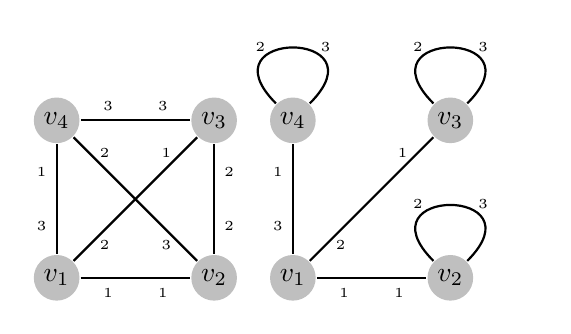
\begin{tikzpicture}[line join=bevel, thick, every loop/.style={}]
  \tikzstyle{vertex}=[circle,fill=black!25,minimum size=12pt,inner sep=2pt]
  \tikzstyle{edge_label}=[font=\tiny]
  \node[vertex] (1) at (0,0)  {$v_1$};
  \node[vertex] (2) at (2,0)  {$v_2$};
  \node[vertex] (3) at (2,2)  {$v_3$};
  \node[vertex] (4) at (0,2)  {$v_4$};
  \node[vertex] (1b) at (3,0)  {$v_1$};
  \node[vertex] (2b) at (5,0)  {$v_2$};
  \node[vertex] (3b) at (5,2)  {$v_3$};
  \node[vertex] (4b) at (3,2)  {$v_4$};
  \path (1) edge node [edge_label, near start, below] {1} node [edge_label, near end, below] {1} (2)
        (1) edge node [edge_label, near start, below] {2} node [edge_label, near end, above] {1} (3)
        (1) edge node [edge_label, near start, left] {3} node [edge_label, near end, left] {1} (4)
        (2) edge node [edge_label, near start, right] {2} node [edge_label, near end, right] {2} (3)
        (2) edge node [edge_label, near start, below] {3} node [edge_label, near end, above] {2} (4)
        (3) edge node [edge_label, near start, above] {3} node [edge_label, near end, above] {3} (4);

  \path (1b) edge node [edge_label, near start, below] {1} node [edge_label, near end, below] {1} (2b)
        (1b) edge node [edge_label, near start, below] {2} node [edge_label, near end, above] {1} (3b)
        (1b) edge node [edge_label, near start, left] {3} node [edge_label, near end, left] {1} (4b)
        (2b) edge [loop] node [edge_label, near start, above] {3} node [edge_label, near end, above] {2} (2b)
        (3b) edge [loop] node [edge_label, near start, above] {3} node [edge_label, near end, above] {2} (3b)
        (4b) edge [loop] node [edge_label, near start, above] {3} node [edge_label, near end, above] {2} (4b);

\end{tikzpicture}
\end{center}

Universal Traversal Sequence: $(1, 2, 3, 2, 1, 1, 2, 1, 3, 1, 2)$

\end{frame}

\section{Space-Complexity}\label{space-complexity}

\begin{frame}{Space-Complexity classes L and NL}

\begin{itemize}
\item
  Input already occupies $n$ cells.
\item
  Seperate space usage of input/output from computation
\item
  We need a different turing machine model, with 3 tapes:

  \begin{itemize}
  \itemsep1pt\parskip0pt\parsep0pt
  \item
    1 read-only input tape
  \item
    1 read/write work tape
  \item
    1 write-only output tape
  \end{itemize}
\item
  Head of input tape \emph{must} remain on the input (+ a
  \emph{constant} offset)
\item
  $L = DSPACE(\log n)$
\item
  $NL = NSPACE(\log n)$
\item
  As with $P = NP$, $L = NL$ is also still unknown
\end{itemize}

\end{frame}

\begin{frame}{Examples for problems that can be solved in $L$}

\begin{description}
  \item[\textit{Counting all occurences of a symbol in the input}] \hfill \\
    $\log n$ bits for the current count
  \item[\textit{Maximum distance between symbols}] \hfill \\
    counter for current distance and current maximum
  \item[\textit{Write down all positions of a certain symbol}] \hfill \\
    counter for current position. The output is in $O(n \cdot \log n)$
\end{description}

\end{frame}

\begin{frame}{$NL \subseteq P$}

\begin{theorem}
The running time of every decider for a problem in L or NL is bounded by a polynominal.
\end{theorem}

\begin{itemize}
\item Configuration:
    \[
        c = (\overbrace{p_i}^{\text{input head position}}, \underbrace{p_w}_{\text{working head position}}, \overbrace{T}^{\text{tape state}}, \underbrace{q}_{\text{state(s)}})
    \]
\item Number of possible configurations:
$$
\begin{array}{rcl}
n_{p_i} \cdot n_{p_w} \cdot n_T \cdot n_q & = & (n + c_1) \cdot (\log n + c_2) \cdot \Gamma^{\log n + c} \cdot c_q \\
                                          & < & (n + c_1) \cdot (\log n + c_2) \cdot n^k \in O(n^{k+2}) \\
\end{array}
$$
\item Construct \textbf{deterministic TM} for a fixed L or NL decider and compute \textbf{next configuration} until
        a \textbf{halting state} is reached.
\end{itemize}

\end{frame}

\begin{frame}{NL-completeness}

\begin{itemize}
\item
  Similar to NP-completeness (just with a space-bound)
\item
  Use a decider for problem $A$ to decide any other problem $B$ in $NL$
\item
  We need a \textbf{transformation function} for instances of $B$ to $A$
\item
  Transformation function needs a logarithmic space bound as well
\end{itemize}

\end{frame}

\begin{frame}{PATH is NL-complete}

\begin{theorem}
    PATH is NL-complete.
\end{theorem}

\begin{proof}
\begin{itemize}
    \item $PATH \in NL$: Non-deterministically \textbf{guess} a path (we have an upper bound on the \textbf{path length}, so we \textbf{always halt}).
    \item Transform \textbf{decider} for $B$ into (directed!) \textbf{graph of configurations}
    \item Add \textbf{single} \textit{accepting node} from all configurations that have an accepting state
    \item Apply $PATH$ to check for a \textbf{path} from the \textit{start configuration} to the \textit{accepting node}
\end{itemize}
\end{proof}

\end{frame}

\section{RL and RandomWalk}\label{rl-and-randomwalk}

\begin{frame}{RL}

\begin{itemize}
\item
  Deciders: Turing machines with \textbf{logarithmic space bound},
  \textbf{polynomial running time} and capable of \textbf{random
  decisions}

  $x \in A \Rightarrow Pr[M \text{ accepts } x] \geq \frac{1}{2}$

  $x \not \in A \Rightarrow Pr[M \text{ accepts } x] = 0$
\item
  Important: Randomization $\not =$ Non-Determinism
\item
  But easy to see that $L \subseteq RL \subseteq NL$
\item
  We actually need the \textbf{polynominal running time} here, since
  randomization breaks our upper bound on running time
\end{itemize}

\end{frame}

\begin{frame}{$UPATH \in RL$, RandomWalk}

\begin{theorem}
$UPATH \in RL$
\end{theorem}

\renewcommand{\algorithmicrequire}{\textbf{Input:}}
\renewcommand{\algorithmicensure}{\textbf{Output:}}

\begin{algorithmic}
\Require $(G, a, b)$
\State $v \gets a$
\For{$i \gets 1$ to \clr{green!80!black}{$p(n)$}}
    \State Randomly select a node $w$ that is adjacent to $v$
    \State $v \gets w$
    \If{$v = b$}
        \State {\bf accept.}
    \EndIf
\EndFor
\State {\bf reject.}
\end{algorithmic}

Find a \textbf{polynom} \clr{green!80!black}{$p(n)$} that
\textbf{guarantees} us to correctly accept with \textbf{probability of
at least $\frac{1}{2}$} if $(G, a, b) \in UPATH$

\end{frame}

\begin{frame}{RandomWalk does not solve PATH}

Example graph for $n=4$.

\begin{center}
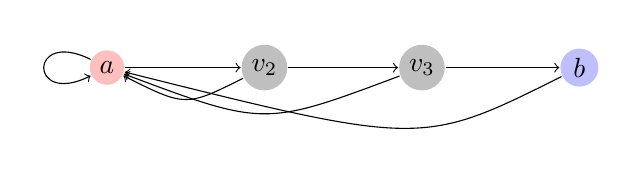
\begin{tikzpicture}[line join=bevel]
  \tikzstyle{vertex}=[circle,thick,fill=black!25,minimum size=12pt,inner sep=2pt]
  \node[vertex, fill=red!25] (G_1) at (-2,0) {$a$};
  \node[vertex] (G_2) at (0,0)  {$v_2$};
  \node[vertex] (G_3) at (2,0)   {$v_3$};
  \node[vertex, fill=blue!25] (G_4) at (4,0)   {$b$};
  \draw [->] (G_1) -- (G_2);
  \draw [->] (G_2) -- (G_3);
  \draw [->] (G_3) -- (G_4);
  \draw [->] (G_1) .. controls (-3.0, 0.5) and (-3.0, -0.5).. (G_1);
  \draw [->] (G_2) .. controls (-1.0, -0.5) .. (G_1);
  \draw [->] (G_3) .. controls (0.0, -0.75) .. (G_1);
  \draw [->] (G_4) .. controls (2.0, -1.0) .. (G_1);
\end{tikzpicture}
\end{center}

For graphs of this form the \textbf{expected number of trials} $E(T)$
before we reach \clr{blue}{$b$} starting at \clr{red}{$a$} is $2^{n}$.

\[
\left.
\begin{array}{rcl}
\frac{1}{2} & = & Pr[T < x] \\
            & = & 1 - Pr[T \geq 2^k] \\
            & \leq & 1 - \frac{E(T)}{x} \\
            & = & 1 - \frac{2^n}{x} \\
\frac{2^n}{x} & \leq & \frac{1}{2} \\
x & \geq & 2^{n+1} \\
\end{array}
\right\}
\begin{array}{l}
\text{At least } 2^{n+1} \text{ steps}\\
\text{needed for correct RL decider.}
\end{array}
\]

\end{frame}

\begin{frame}{Expected number of steps from $a$ to $b$}

\begin{block}{Important}
We assume that $G$ is \textbf{connected} here, since we only care about
the \textbf{number of steps} we need to take if \clr{red}{$a$} and \clr{blue}{$b$}
actually are in the \textbf{same connected component}.
\end{block}

\end{frame}

\begin{frame}{Markov-Chains and RandomWalk}

Markov-Chain:

\begin{itemize}
\itemsep1pt\parskip0pt\parsep0pt
\item
  Chain of random variables $X_i$, that have the \emph{markov property}
\item
  $X_i \in S$ models that we are in state $s \in S$ at step $i$
\item
  Distribution over states: Probability that we are in each state
\item
  Transition probabilities between states
\end{itemize}

Model a \emph{RandomWalk} on $G = (V, E)$ as Markov-Chain with
\emph{finite} states:

\begin{itemize}
\item
  Nodes $V$ are the states
\item
  Transition probability for $u$ to $v$:

  \[ Pr[X_i = v | X_{i-1} = u] = \left\{
    \begin{array}{l l}
      \frac{1}{d(u)} & \quad \text{if $v$ is adjacent to $u$}\\
      0 & \quad \text{otherwise}
    \end{array} \right.
  \]
\end{itemize}

\end{frame}

\begin{frame}

Graph and corresponding state space with transition probabilities.

\begin{center}
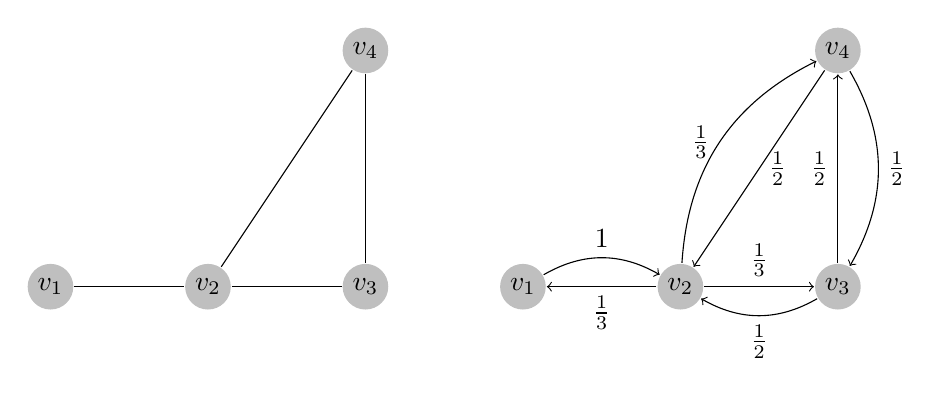
\begin{tikzpicture}[line join=bevel]
  \tikzstyle{vertex}=[circle,thick,fill=black!25,minimum size=12pt,inner sep=2pt]
  \node[vertex] (G_1) at (-2,0)  {$v_1$};
  \node[vertex] (G_2) at (0,0)   {$v_2$};
  \node[vertex] (G_3) at (2,0)   {$v_3$};
  \node[vertex] (G_4) at (2,3)   {$v_4$};
  \draw (G_1) -- (G_2);
  \draw (G_2) -- (G_3);
  \draw (G_2) -- (G_4);
  \draw (G_3) -- (G_4);

  \node[vertex] (H_1) at (4,0)  {$v_1$};
  \node[vertex] (H_2) at (6,0)   {$v_2$};
  \node[vertex] (H_3) at (8,0)   {$v_3$};
  \node[vertex] (H_4) at (8,3)   {$v_4$};
  \path (H_1) edge [->, bend left] node[above] {1} (H_2)
        (H_2) edge [->] node[below] {$\frac{1}{3}$} (H_1)
        (H_2) edge [->] node[above] {$\frac{1}{3}$} (H_3)
        (H_3) edge [->, bend left] node[below] {$\frac{1}{2}$} (H_2)
        (H_2) edge [->, bend left] node[left] {$\frac{1}{3}$} (H_4)
        (H_4) edge [->] node[right] {$\frac{1}{2}$} (H_2)
        (H_3) edge [->] node[left] {$\frac{1}{2}$} (H_4)
        (H_4) edge [->, bend left] node[right] {$\frac{1}{2}$} (H_3);
\end{tikzpicture}
\end{center}

\[
\nu = (1, 0, 0, 0), 
P =
\begin{pmatrix}
0 & 1 & 0 & 0 \\
\frac{1}{3} & 0 & \frac{1}{3} & \frac{1}{3} \\
0 & \frac{1}{2} & 0 & \frac{1}{2} \\
0 & \frac{1}{2} & \frac{1}{2} & 0 \\
\end{pmatrix},
\begin{matrix}
\nu  \cdot P & = & (0, 1, 0, 0) \\
\nu \cdot P^2 & = & (\frac{1}{3}, 0, \frac{1}{3}, \frac{1}{3}) \\
\end{matrix}
\]

\end{frame}

\begin{frame}{From Markov Chains to expected number of steps}

\begin{theorem}
The expected number of steps $E(v, v)$ of a node $v \in V$ to reoccur is $\frac{2e}{d(v)}$,
where $e = |E|$.
\end{theorem}

\begin{proof}
\begin{enumerate}
\item Proof that our markov chain is \textbf{irreducible} and \textbf{time-homogenous}.
\item Proof that $\pi = (\frac{d(v_0)}{2e}, \cdots, \frac{d(v_n)}{2e})$ is the stationary distribution: $\pi = \pi \cdot P$
\item Proof that if we choose the start node \textbf{uniformly distributed} we will converge on the stationary distribution.
\item Expected number of steps before a state $v$ reoccures is $\frac{1}{\pi(v)} = \frac{2e}{d(v)}$
\end{enumerate}
\end{proof}

\end{frame}

\begin{frame}{From Markov Chains to expected number of steps}

\begin{theorem}
The expected number of steps $E(a, G)$ to reach all nodes in G starting at a node $a$ is less than $4 \cdot e \cdot n$.
\end{theorem}

\begin{proof}
\begin{enumerate}
\item The expected number of steps $E(u, v)$ of an edge $\{u, v\} \in E$ to reoccur is less than $2e$:
      $E(u, v) \leq E(u, u) \cdot \frac{1}{d(u)}$
\item There is always a path of length at most $2n$ that visits all nodes.
\end{enumerate}
From that we can estimate $E(a, G)$ with a path $(v_1, \dots, v_k)$ ($k \leq 2n$) that visits all nodes in $G$:
$$
E(a, G) \leq \sum_{i=1}^{k} E(v_{i-1}, v_i) < 2n \cdot 2e = 4en
$$
\end{proof}

\begin{proof}
At node $u$ the probability to select $v$ is $\frac{1}{d(u)}$, the number of steps to get back at $u$ is $E(u, u)$.
Thus $E(u, v) \leq E(u, u) \cdot \frac{1}{d(u)}$
\end{proof}

\end{frame}

\begin{frame}{From Markov Chains to expected number of steps}

\begin{theorem}
The probability to reach \clr{blue}{$b$} from \clr{red}{$a$} using $8en$ steps is higher than $\frac{1}{2}$.
\end{theorem}

\begin{proof}
Let $T(a, b)$ be the number of steps from $a$ to $b$.
$$
Pr[T(a, b) \geq 8en] < \frac{E(a, b)}{8en}
                     < \frac{E(a, G)}{8en}
                     < \frac{4en}{8en} = \frac{1}{2}
$$
$$
Pr[T(a, b) < 8en] = 1 - Pr[T(a, b) \geq 8en]
                  < 1 - \frac{1}{2} = \frac{1}{2}
$$
\end{proof}

\end{frame}

\section{Universal Traversal
Sequences}\label{universal-traversal-sequences}

\begin{frame}{RandomWalk $\leftrightarrow$ Universal Traversal Sequence}

\begin{itemize}
\itemsep1pt\parskip0pt\parsep0pt
\item
  From the $UPATH \in RL$ proof: $E(a, G) \leq 8en$
\item
  After $E(a, G)$ steps the probability to \textbf{not} visit all nodes
  is less than $\frac{1}{2}$
\end{itemize}

Probability amplification:

\begin{itemize}
\itemsep1pt\parskip0pt\parsep0pt
\item
  Repeat multiple times to increase propability that we did visit all
  nodes
\item
  Probability that we did not visit all nodes after $m$ tries: $2^{-m}$
\item
  Length of random walk $8en \cdot m$
\item
  Probability increases \textbf{exponential} for \textbf{polynomial}
  increase in length
\end{itemize}

\end{frame}

\begin{frame}{On d-regular Graphs}

\begin{itemize}
\item
  $d$-regular Graph: Each node has degree $d$.
\item
  Traversal sequence: $(i_1, ... , i_k), i_j \in \{0, \dots, d-1\}$
\item
  RandomWalk in d-regular graph: Choose $i_j$ uniformly distributed
\item
  There are less than $n^{n \cdot d} =: g_{n,d}$ $d$-regular graphs of
  size n.
\item
  Idea: Make $m$ big enough that the probability of a given traversal
  sequences to work for all graphs is bigger than 0:
\end{itemize}

If $F$ is the number of for which a traversal sequence does not work.

$E(F) = g_{n, d} \cdot 2^{-m} < 1$, thus:

\[
\left.
\begin{array}{rcl}
1 - Pr[F < 1] & = & Pr[F \geq 1] \\
              & \leq & \frac{E(F)}{1} < 1 \\
\Rightarrow 0 & < & Pr[F < 1] \\
\end{array}
\right\}
\text{Works for } m > \log_2 n \cdot nd
\]

\end{frame}
